\documentclass[UTF8,10pt,a4paper]{ctexart}
\usepackage[utf8]{inputenc}
\usepackage{amsmath}
\usepackage{amsfonts}
\usepackage{amssymb}
\usepackage{graphicx}
\usepackage{geometry}


\author{陈斯杰}
\title{Chapter1. THE GENESIS OF FOURIER ANALYSIS}
\begin{document}
\maketitle
\begin{abstract}
This book begins the talk of Fourier Analysis with two 
physical problem: vibrating string and heat conduction.
In this review, I am going to illustrate these two examples
in detail by supplementing the background knowledge.
\end{abstract}

\section{The Vibrating String}
	\subsection{Simple harmonic motion 简谐运动}
		\begin{figure}[ht]
			\centering
			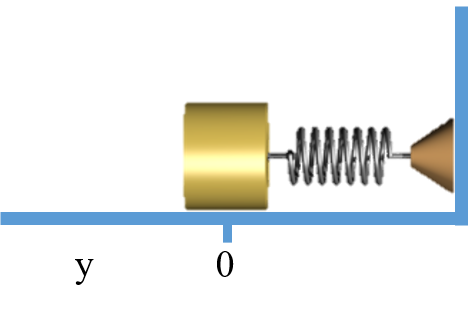
\includegraphics[width=5cm]{idealspring.png}
			\caption{简谐运动谐振子}
			\label{fig:simple_harmonic}
		\end{figure}
		
		\noindent
		Newton's law produces a 2nd order ODE

		\begin{equation}
			F=-ky(t) \Rightarrow -ky(t)=my''(t)
		\end{equation}

		Let $c=\sqrt{\frac{k}{m}}$, we get a neater form: 
		
		\begin{equation}
			y''(t)+c^2y(t)=0
		\end{equation}				
		\noindent
		Equation(2)	is a linear homogeneous 2nd-order differential equation(二阶常系数线性方程).
		For a general case $y''+py'+qy=0$, we first solve the characteristic equation
		$\lambda^2+p\lambda+q=0$ and get the characteristic roots: $\lambda_1, \lambda_2$.
		
		\begin{tabular}{|lll|}
		\hline
		Characteristic Roots & Linear Independent Sol. Pair & General Sol.\\
		\hline
		$\lambda_1,\lambda_2\in\mathbb{R}\ and\ \lambda_1\neq\lambda_2$ &
		$y_1=e^{\lambda_1 x}, y_2=e^{\lambda_2 x}$ &
		$y=C_1e^{\lambda_1 x}+C_2e^{\lambda_2 x}$ \\
		
		$\lambda_1,\lambda_2\in\mathbb{R}\ and\ \lambda_1=\lambda_2$ &
		$y_1=e^{\lambda_1 x}, y_2=xe^{\lambda_1 x}$ &
		$y=(C_1+C_2x)e^{\lambda_1 x}$ \\
		
		$\lambda_1,\lambda_2=\alpha\pm i\beta$ &
		$y_1=e^{\alpha x}\cos\beta x, y_2=e^{\alpha x}\sin\beta x$ &
		$y=e^{\alpha x}(C_1 \cos\beta x +C_2 \sin\beta x)$ \\
		\hline
		\end{tabular}
    	\  \\
    	\ \\
		The corresponding characteristic equation of (2) is $\lambda^2 + c^2=0$, and the roots
		are $\lambda=\pm ic$; therefore, the general solution of (2) is 
		\begin{equation}
			y(t)=a\cos ct+b\sin ct
		\end{equation}
		and it's 1st order derivative is
		\begin{equation}
			y'(t)=-ac\sin ct +bc\cos ct
		\end{equation}
		To get the particular solution, we need 2 initial condition: $y(0)\ and\ y'(0)$.\\
		$y(0)=a,\ y'(0)=bc$, thereby getting the particular solution:
		\begin{equation}
			y(t)=y'(0)\cos ct + \frac{y'(0)}{c} \sin ct
		\end{equation}
	\subsection{Standing Wave 驻波}
		\begin{figure}[ht]
			\centering
			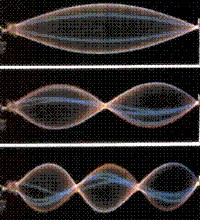
\includegraphics[width=5cm]{standingwave.png}
			\caption{驻波}
			\label{fig:standingWave}
		\end{figure}
		\noindent
		驻波是两个振幅、波长、频率都相同的正弦波,相向而行形成的。
		驻波的波形并不前进,波形上的每个质点皆作Simple Harmonic Motion(简谐运动)。\\
		We use $u(x,t)$ to describe the standing wave. The nature of standing waves suggest 
		the mathematical idea of "separation of variables".\\
		\noindent
		As standing waves do not travel, every mass point just oscillates around the balance position 
		at different amplitudes. So the equation of standing wave movement can be expressed as:
		\begin{equation}
		u(x,t)=\phi (x) \psi(t)
		\end{equation}
		where:\\
		 	$\phi(x)$ represents the amplitute of the mass points at location x. \\
		 	$\psi(t)$ is a oscillating factor, which makes every mass point 
			oscillates within the amplitute $\phi(x)$.
			  
		拨动两端固定并拉紧的弦,机械波经过两固定端的反射,反射的波叠加可形成驻波。
		  
		下面推导弦上的驻波方程:

  		\noindent
  		We subdivided the string into a large number $N$ of mass points, distributed 
  		uniformly along the $x$-axis.\\
  		Each particle's position is $(x_n,y_n)$	, where:
		\begin{equation}
		    \left\{
			\begin{aligned}
				&x_n =nh=n\frac{L}{N} \\
				&y_n(t) =u(x_n,t) \\
			\end{aligned}
			\right.
		\end{equation}
		
		\begin{figure}[ht]
			\centering
			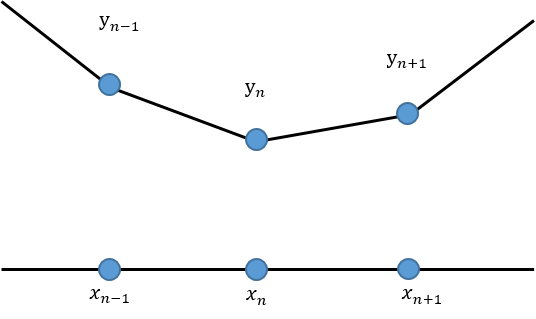
\includegraphics[width=6cm]{vibratingString.png}
			\caption{A Vibrating String}
			\label{fig:vibStr}
		\end{figure}		
  		
		There are two forces acted upon the particle by two neighbour particles;
		i.e. the sum of forces on $(x_n,y_n)$ is $F_l+F_r$.\\
		\begin{figure}[ht]
			\centering
			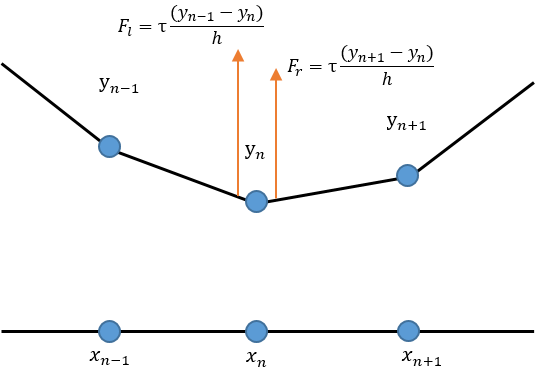
\includegraphics[width=6cm]{vibratingStringF.png}
			\caption{Forces on the string's particle}
			\label{fig:vibStrF}
		\end{figure}
		
		
		\noindent		  
		Now we are going to illustrate why $F_r$ equals  $\tau\frac{(y_{n+1}-y_n)}{h}$. 
		As the particle only oscillates in the y-direction, the horizontal net force is zero.\\		 
		\begin{figure}[h]
			\centering
			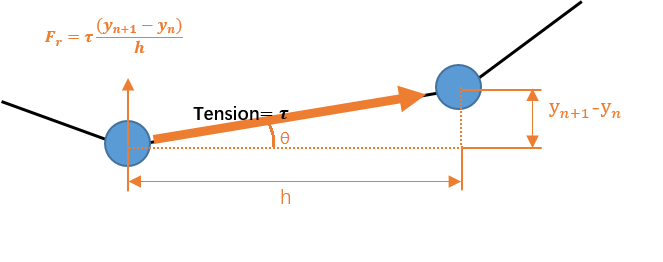
\includegraphics[width=11cm]{tension.png}
			\caption{Force Analysis}
			\label{fig:tens}
		\end{figure}	
		
		
		\noindent
		The y-direction force is the y-component of the tension $\tau$ between the particle and 
		the next particle.\\
		$F_r$ equals $\tau \sin\theta$ ($\theta$ is the angle between the tension and the horizontal line),
		Considering $\theta$ is very small, we substitute $\sin\theta$ with $\tan\theta$.\\
		Hence, $F_r$ approximately equals to $(\tau \tan\theta)= (\tau\frac{(y_{n+1}-y_n)}{h})$ 
		
		
		
		\noindent
		The linear density of the string is $\rho$, so each particle's mass is $\rho h$
		According to Newton's law $F=ma$, we derive the following equation.
		
		\begin{align*}
		\rho h y_n''(t) &= F_l+F_r \\
                        &= \tau\frac{\ y_{n+1}(t)-y_{n}(t)+y_{n-1}(t)-y_n(t)}{h} \\
                        &= \tau\frac{\ u(x_n+h,t)-u(x_n,t)+u(x_n-h,t)-u(x_n,t)}{h}  \\
                        &= \tau\frac{\ u(x_n+h,t)+u(x_n-h,t)-2u(x_n,t)}{h}  \\                        
		\end{align*}
		Let's take the limit of this equation's right side with respect to h,
		\begin{align*}
			\rho h y_n''(t) = \lim_{h\to 0}\tau\frac{\ u(x_n+h,t)+u(x_n-h,t)-2u(x_n,t)}{h} 
		\end{align*}
		\noindent
		and move h to the right side, and use $u(x,t)$ notation to substitute $y{''}(t)$
		\begin{equation}
			\rho \frac{\partial^2 u}{\partial t^2} = \lim_{h\to 0}\tau\frac{\ u(x_n+h,t)+u(x_n-h,t)-2u(x_n,t)}{h^2} 
		\end{equation}
		\noindent
		The right side is right the definition of 2nd order partial derivatives of $u$ with respect to $x$, 
		so in short:
		\begin{equation}
			\frac{1}{c^2}\frac{\partial^2 u}{\partial t^2}=\frac{\partial^2 u}{\partial x^2},\ with\ c=\sqrt{\tau/\rho}
		\end{equation}
		This relation is known as 1-D wave equation, $c>0$ is called the \textbf{velocity} of the motion.\\
		We can examine c's physical meaning using Dimensional Analysis (量纲分析).\\
		The Unit of c is $(N \bullet \frac{kg}{m})^{0.5}=(kg \bullet m/s^2 \bullet \frac{kg}{m})^{0.5}=m/s$
	\subsection{Solving Wave Equation}
		For simplicity, we assume that $c=1$ and length of string $L=\pi$, so Equation (9) becomes
		\begin{equation}
			\frac{\partial^2 u}{\partial t^2} = \frac{\partial^2 u}{\partial x^2}\ (0\leqslant x \leqslant \pi,\ t\geqslant 0)
		\end{equation}				
		
		\subsubsection{using travelling waves}
		我们用$F(x)$来表示某一时刻的波形,$F(x+vt)$则表示$t$个时间后的波形(假设波向右移动)。
		\subsubsection{using the superposition of standing waves}
\end{document}